\section{Theorie}
\label{sec:Theorie}

\subsection{Reflexion und Brechungsindex}
\label{theo1}

Trifft Röntgenstrahlung aus dem Vakuum auf ein Medium mit einem Brechungsindex $n \neq 1$ ist der Brechungsindex gegeben als
\begin{equation}
    n = 1 −  \delta + i \cdot \beta.
    \label{eq:index}
\end{equation}
Dabei ist $\delta$ eine kleine Korrektur $\delta = 10^(-6)$ und $\beta$ die Absorption.
Für Röntgenstrahlen ist der Brechungsindex in Materie kleiner als 1, sodass Totalrelflexion möglich wird.
Zunächst betrachten wir allerdings eine allgemeine Reflexion.
Eine elektromagnetische Welle trifft unter einem Winkel $\alpha_\text{i}$ auf eine homogene, unendlich dicke und glatte Schicht.
Dort wird ein Teil der Welle unter dem Winkel $\alpha _\text{f} = \alpha _\text{i}$ reflektiert und der andere Teil um den Winkel $\alpha _\text{f}$ transmittiert und gebrochen.
Die Reflexion und Transmission ist in \autoref{fig:theo1}

\begin{figure}
    \centering
    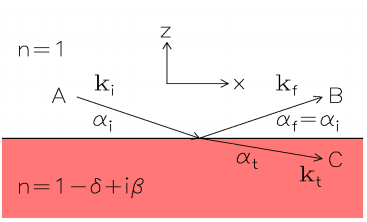
\includegraphics[width=0.5\textwidth]{images/reflektion.png}
    \caption{Darstellung der Reflexion und Transmission einer Welle. \cite{V44-old}}
    \label{fig:theo1}
\end{figure}

Wie bereits besprochen ist hier unterhalb eines bestimmten kritischen Winkels $\alpha _\text{c}$ Totalrelflexion möglich, das bedeutet, dass kein Teil der Welle transmittiert.
Dieser Winkel ist näherungsweise gegeben durch
\begin{equation}
    \alpha _\text{c} = \sqrt{2 \cdot \delta}.
    \label{eq:krit}
\end{equation}
Wird nun die Definition von $\delta$ verwendet, ergibt sich $\alpha _c$ als 
\begin{align}
    \delta &= \frac{\lambda ^2 \cdot r_\text{e} \cdot \rho}{2 \, \pi} \\
    \alpha _\text{c} &=  \lambda  \cdot \sqrt{\frac{r_\text{e} \cdot \rho}{\pi}}
\end{align}

In den Fresnelschen Gleichungen wird zudem die Polarisation der Wellen betrachtet, allerdings sind die Gleichungen für Röntgenstrahlen gleich, da die beiden $n$ nahezu 1 sind.
Dadurch ergeben sich die klassichen Fresnel-Gleleichungen als
\begin{align}
    t &= \frac{2 \, N_1 \, \sin{\alpha _\text{i}} }{N_1 \, \sin{\alpha _\text{i}} + N_2 \, \sin{\alpha _\text{t}}} \\
    r &= \frac{N_1 \, \sin{\alpha _\text{i}} - N_2 \, \sin{\alpha _\text{t}}}{N_1 \, \sin{\alpha _\text{i}} + N_2 \, \sin{\alpha _\text{t}}}.
\end{align}
Dabei sind $r$ und $t$ die Fesnel'schen Reflexions- und Transmissionskoeffizienten. 
Diese stellen Amplitudenverhältnisse dar, wir sind eher an Intensitätsverhältnissen interessiert.
Daher betrachten wir die Fresnel'sche Reflektivität unter der Annahme, dass $\alpha _\text{i} > 3 \, \alpha _\text{c}$ als 
\begin{equation}
    R_\text{F} = |r|^2 = \left( \frac{{\alpha _\text{c}}^4}{2 \, \alpha _\text{i}}  \right).
    \label{eq:reflek}
\end{equation}

\subsection{Mehrschichtsysteme}
\label{theo2}

In der Realitiät sind Systeme aber selten homogen und einschichtig, daher betrachten wir jetzt die Reflexion an einer Probe mit Schicht.
Als Beispiel soll ein Silizium-Wafer mit einer $\SI{800}{\angstrom}$ dicken Polystyrolschicht dienen. 
Trägt man die Reflektivität gegen den Einfallswinkel auf ergibt sich ein Plot wie in \autoref{fig:theo2}.

\begin{figure}
    \centering
    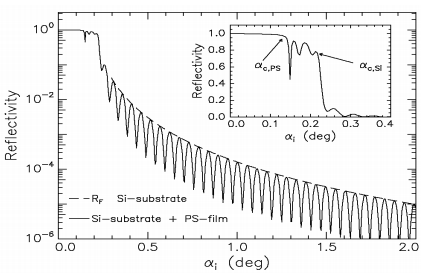
\includegraphics[width=0.5\textwidth]{images/plot.png}
    \caption{Reflektivität in Abhängigkeit vom Einfallswinkel bei unserem Beispiel. \cite{V44-old}}
    \label{fig:theo2}
\end{figure}

Die gestrichelte Linie stellt die theoretische Fresnelreflektivität dar.
Es ist allerdings zu erkennen, dass sie in der Realität oszilliert, dies sind die sogenannten Kiessig-Oszillazionen. 
Sie entstehen durch Interferenz an den Grenzflächen, die je nach Phasendifferenz konstruktiv oder destruktiv ist.
Die Minima entsehen, wenn sich zwei Wellen auslöschen, das geschieht bei einem Gangunterschied von $ n \cdot \frac{\lambda}{2}$, wobei $n$ eine ungerade Zahl ist.
Bei den kritischen Winkeln beider Schichten sind klare Einbrüche im Plot zu erkennen. 
So ergeben sich die Werte
\begin{align}
    \alpha _\text{c,PS} &= \SI{0.15}{\degree} \\
    \alpha _\text{c,SI} &= \SI{0.22}{\degree}
\end{align}
Über die Wellenlänge $\lambda$, der Oszillazion, kann dann die Schichtdicke $d$ als 
\begin{equation}
    d = \frac{\lambda}{2 \, \Delta \alpha _\text{i}}
    \label{eq:schicht}
\end{equation}
berechnen.

Sollte es noch viele weitere Schichten geben, werden die Oszillazionen überlagert und es ist kompliziert etwas über die einzelnen Schichten auszusagen.
Dafür gibt es den sogenannten Parrat-Algorithmus, dieser basiert auf einem rekursiven Durchlaufen durch alle Schichten.
Angefangen wird dabei mit der unterrsten Schicht.
Allerdings wird in diesem Versuch nur eine Schicht vorkommen, daher ist ein tieferes Verständnis des Algorithmus hier nicht notwendig.

Eine weitere Korrektur ist noch nötig, die Rauigkeitskorrektur. 
Glatte Oberflächen treten in der Natur nicht wirklich auf, daher wird eine "root-mean-square“ (rms) – Rauigkeit der j-ten Grenzfläche eingeführt.
Mit Hilfe dieser werden die Fresnelkoeffizienten modifiziert.
Diese können dann im Parratt-Algorithmus verwendet werden, ansonsten bleibt die Rechnung die gleiche.

\subsection{Funktionsweise der Geräte im Versuch}
\label{theo3}
 
Die Röntgenstrahlung erhalten wir aus einer Kupfer-Röntgenröhre.